\begin{teamsubmission}{Parse Patrol}{Parse Patrol: Dual-Mode Scientific Parsing Infrastructure via MCP Servers}
\authorsblock{
    Nathan Daelman\textsuperscript{1}\orcidlink{0000-0002-7647-1816},
    Christina Ertural\textsuperscript{2}\orcidlink{0000-0002-7696-5824},
    Rubel Mozumber\textsuperscript{1}\orcidlink{0009-0007-5926-6646},
    Sascha Klawohn\textsuperscript{1}\orcidlink{0000-0003-4850-776X},
    Remya Ann Mathews Kalapurakal\textsuperscript{3} 
}
\affiliationsblock{
    \textsuperscript{1}Humboldt University of Berlin, 10117 Berlin, Germany\\
    \textsuperscript{2}Department of Materials Chemistry, Federal Institute for Materials Research and Testing, 12205 Berlin, Germany\\
    \textsuperscript{3}University of New Hampshire, 03824 Durham, NH, USA
}

\section*{Introduction}

Parsing scientific files to extract structured data depends strongly on specifications.
These specifications may exist at a format level, a schema level, or more abstractly, an ontological one.
This dependency makes parser infrastructure very brittle and labor-intensive to maintain, as changes to either source or target specifications require updating parsers accordingly.
This is a frequent issue in materials and chemistry databases and consortia. 

The rise of large language models (LLMs) has opened up new avenues for automating parser development, as modern models can reason over heterogeneous file formats and dynamically adapt to evolving specifications.
However, effective use of LLMs requires a reliable interface for connecting models to external tools.
Anthropic published the Model Context Protocol (MCP) in late 2024\cite{mcp2024}, providing a standardized interface for agents to discover and invoke external tools, access resources, and use predefined prompts\cite{mcp_def}.
It has since become the industry standard supported by all major commercial models.

In this work, we present Parse Patrol, an AI-assisted workflow for rapidly discovering, testing, and deploying parsers that conform to user-defined specifications.
Parse Patrol leverages MCP to integrate community parsers into a unified interface, enabling agents to iteratively evaluate parser options against target schemas.
The same infrastructure supports two usage modes:
(i) Discovery Mode, where an agent interactively tests parsers for schema conversion;
and (ii) Direct Import Mode, where the same parsers are available as Python modules for production code.

\section*{Results}

Automated parser generation faces several pitfalls:
scarce online resources for scientific specifications, model hallucinations outside training data, lengthy test iterations, and unstable software architectures.
Parse Patrol sidesteps these issues by leveraging community parsers, focusing instead on widening the specification coverage and design options.
Because MCP provides a uniform, model-agnostic interface for invoking software tools, individual parsers can be exposed as MCP tools, allowing agents to orchestrate them seamlessly during parser selection, testing, and schema conversion.

MCP, however, does not prescribe how to organize tools: by default, servers simply expose a flat list of tools.
Our first technical innovation is to define a \textit{hierarchical protocol} for structuring the MCP server.
Each parser is implemented as its own independent MCP server, which enables targeted feature development and testing.
These individual servers' components are then automatically registered with a central, user-facing server.
The central server aggregates all parser tools and resources, then adds prompts for test deployment and production workflows.
The user provides specifications either directly in the chat or as separate files, while test cases can be retrieved via database MCP servers.

While MCP tools enable interactive testing and one-off parsing tasks, bulk processing and production workflows require importable modules.
Parse Patrol addresses this by exposing the same parser both as an MCP server and as a Python module.
To ensure agents leverage these modules when writing code, we employ a two-pronged approach: prompts provide usage instructions, while each parser server exposes its module path and import syntax as an MCP resource.

Implementing this dual-mode design (cf. Fig.\ref{fig:parse-patrol}) is challenging, as MCP servers and Python packages have different distribution requirements.
MCP servers are typically registered in the \href{https://github.com/modelcontextprotocol/servers}{MCP Registry}\cite{mcp2024registry}, while Python packages are distributed via \href{https://pypi.org/}{PyPi}\cite{pypi}.
Parse Patrol bridges this divide by maintaining a unified codebase that satisfies both frameworks' requirements, where each tool's schema serves both modes.
This ensures the tool interfaces evolve with use in both contexts.
To the best of the authors' knowledge, no other framework provides this dual-mode capability.

\begin{figure}[h]
    \centering
    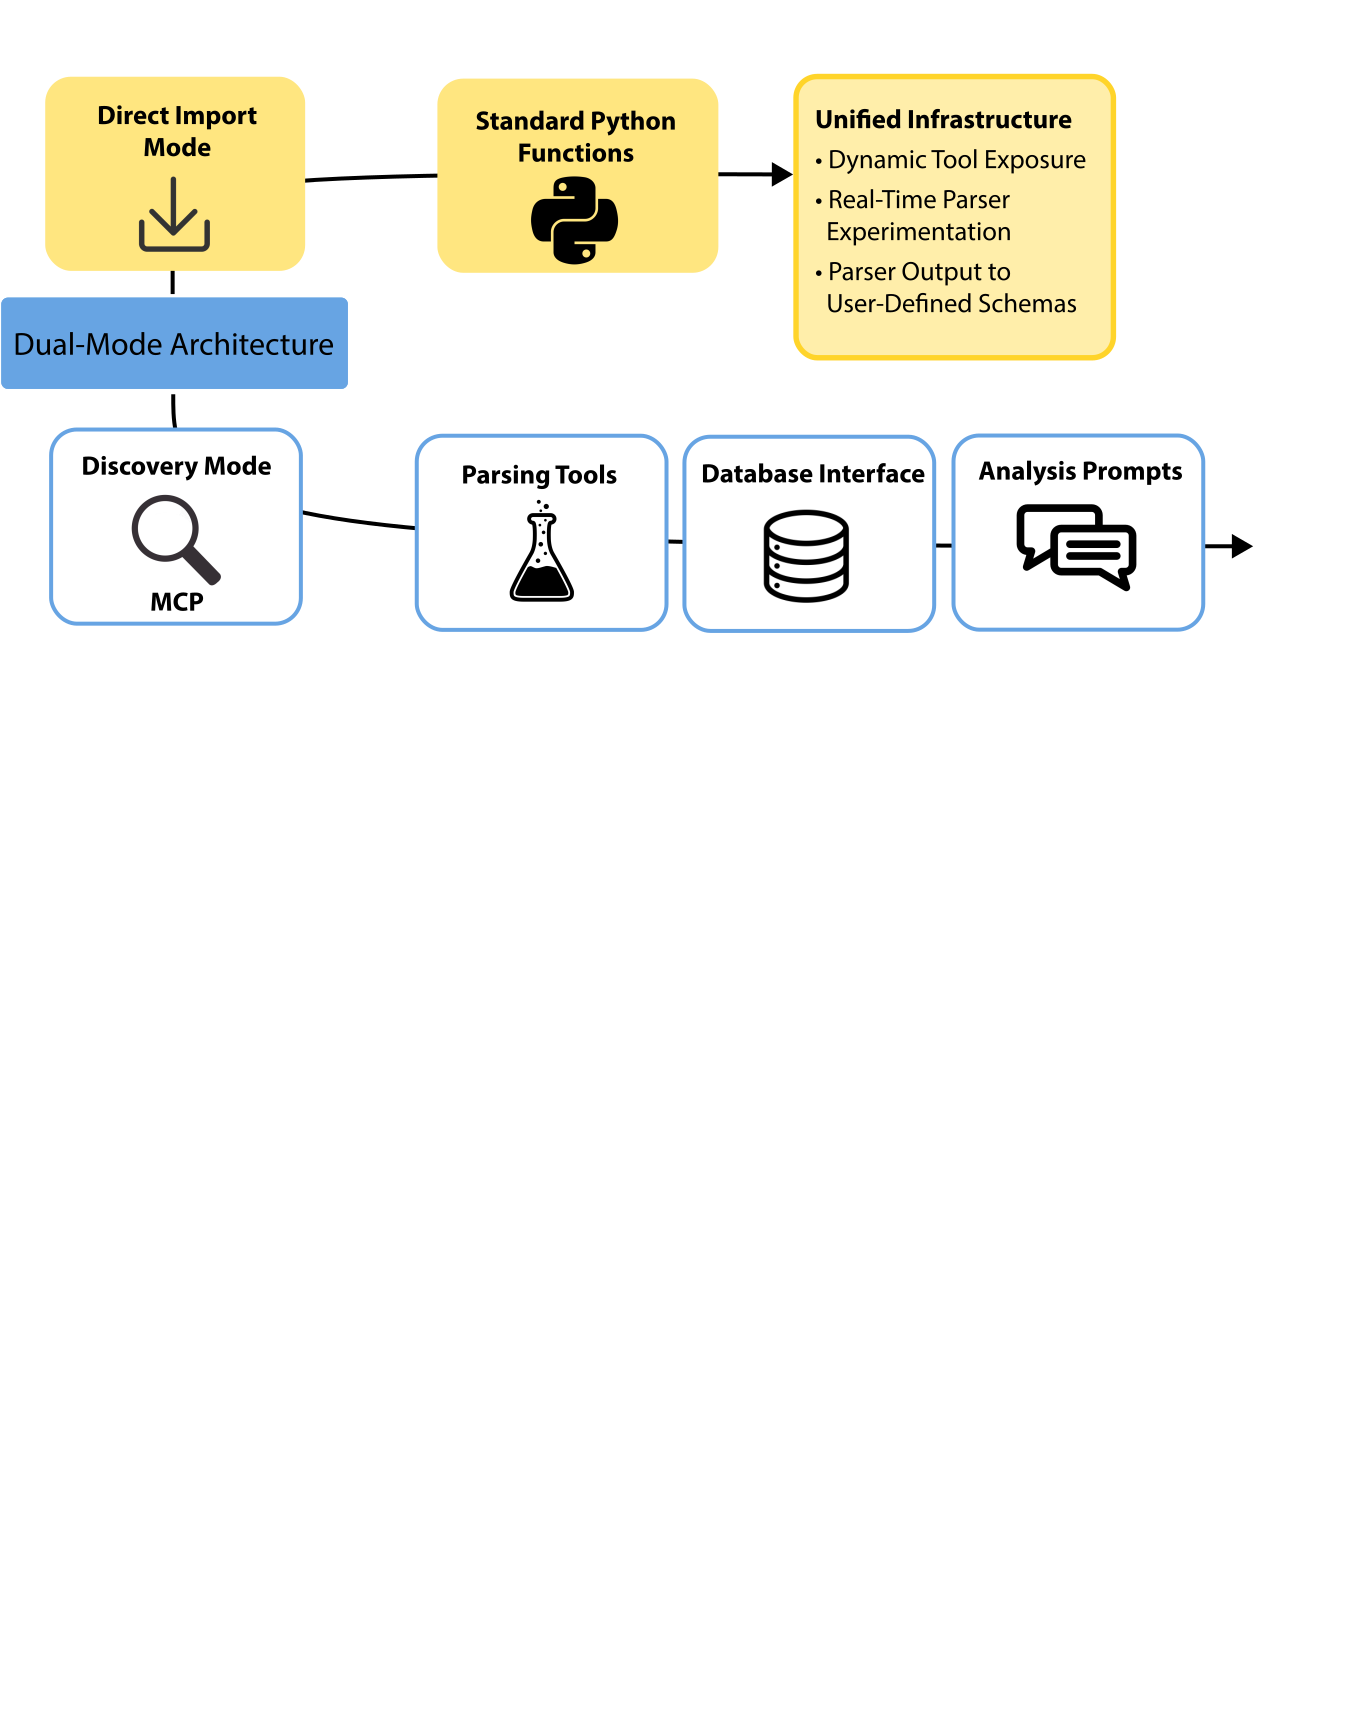
\includegraphics[width=0.8\linewidth]{figures/parse-patrol.png}
    \captionsetup{width=\linewidth}
    \caption{
    Schematic depiction of the \textit{dual-mode} design in Parse Patrol.
    \textbf{Lower branch:} Discovery mode provides a single MCP interface to several parser and database servers.
    The central server further exposes prompts for the suggested use case.
    \textbf{Upper branch:} Direct Import mode exposes the same MCP components as Python modules for friction-less switching from testing to production.
    Both branches are unified under a single architecture.
    }
    \label{fig:parse-patrol}
\end{figure}

\section*{Future Work}

At the time of writing, the repository is seeing active development.
Given the well-defined objective of providing a computational parsers toolkit, future extensions are not excluded.
This project is under consideration for incorporation into NOMAD parser suite\cite{nomad_lab,draxl2019nomad}.

\section*{Open Source Materials}

The open source code is available on GitHub: \github{https://github.com/ndaelman-hu/parse-patrol} (latest development version). For stable releases, consult the version tags. Submitted version for the hackathon: \texttt{v0.0.2-beta}.
A demo video is available on YouTube: \youtube{https://www.youtube.com/watch?v=fSAyi5ubkR0}.

\section*{Author Contributions}

\textbf{N.D.}: Conceptualization, Software, Original Code Draft, Visualization - Writing of Documentation and Manuscript, Editing
\textbf{C.E.}: Conceptualization Revision, Software, Visualization, Video Editing, Writing - Original Manuscript Text Draft, Figure, Editing
\textbf{R.M.}: Implementation asynchronous servers, Extension Testing Infrastructure - Conceptualization Revision, Proof-read Manuscript
\textbf{S.K.}: Extend Parser Servers - Proof-read Manuscript
\textbf{R.A.M.K.}: Testing of Setup, Trial new Parsers - Proof-read Manuscript

\section*{Acknowledgements}
This work was supported by the NFDI consortium FAIRmat - Deutsche Forschungsgemeinschaft (DFG) - Project 460197019.

\end{teamsubmission}
